As introduced in section \ref{SEC:L2PAIRWISE}, the use of the metric $\mathbb{L}^2$
for the pairwise alignment of functions leads to a series of difficulties, which make
it unsuitable for this problem. This is why we will use differential
geometry techniques to find a suitable metric. In particular, given two
functions $f_1$, $f_2$ and $\gamma \in \Gamma$, we look for a metric that
remains invariant to warpings in the domain, i. e.,
$d(f_1, f_2) = d(f_1 \circ \gamma, f_2 \circ \gamma)$.

For this purpose we will use the Fisher-Rao metric. This Riemannian metric was
introduced in 1945 by C. R. Fisher in a version on the
space of probability distributions. In our case we will use a non-parametric
version, slightly different from the original one, defined on the space of
signed measures. This metric plays a very important role in information
geometry, and it is the only metric that possesses this property of
invariance to warpings in the domain\cite{Cencov1982}.

\begin{figure}[Tangent space of tridimensional manifold]{FIG:TANGENT}{Tangent space of tridimensional manifold $M$ \footnotemark}
	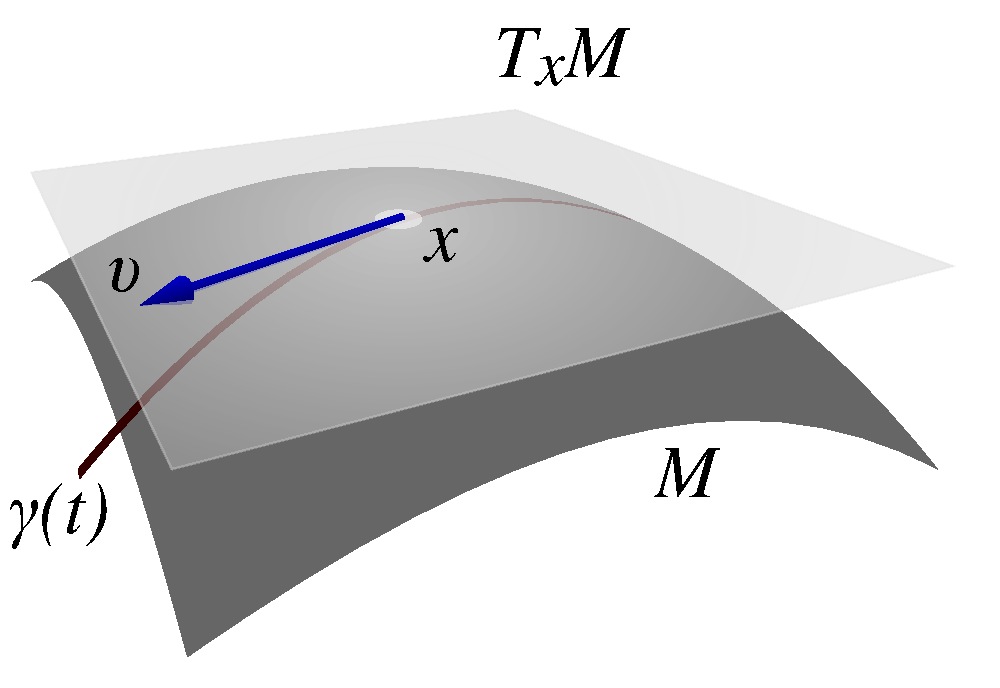
\includegraphics[width=6.5cm]{tangential-vector}
\end{figure}

\footnotetext{Derivative work: McSush. Original uploader: TN at German Wikipedia. [Public domain]}

A Riemannian metric is an application that assigns an inner product at each
point of variety on its tangent space that varies smoothly from point to point.
This will give us local notions of angles, length of curves or volumes.

The tangent space of a manifold facilitates the generalization of
vectorsto general manifolds, since one
cannot simply subtract two points to obtain a vector that gives the displacement
of the one point from the other. The tangent space of a point $x$ in a general
manifold $M$, denoted as $T_xM$, is made up of the velocities at $x$ of all the
paths of the variety passing through the point. For example, in the Figure
\ref{FIG:TANGENT} is shown a manifold $M$ in $\mathbb{R}^3$. This velocities of
the path are tangent vectors to the curve. In this case the tangent space $T_xM$
made up of all these vectors is a plane.



In our case the manifold will be formed by the set of absolutely continuous
functions $\mathcal{F}$, that is, those functions whose derivative exists a.e.
and belongs to the space of square integrable functions $\mathbb{L}^2$. An
the path between points of $\mathcal{F}$ may be understood as smooth
deformations of the functions.
We will endow $\mathcal{F}$ with the Fisher-Rao metric.

Let $f \in \mathcal{F}$  and $v_{1}, v_{2} \in T_{f}(\mathcal{F})$,
the Fisher-Rao metric is defined as

\begin{equation}[EQ:FRAO]{Fisher-Rao metric}
\left\langle\left\langle v_{1}, v_{2}\right\rangle\right\rangle_{f}=
\frac{1}{4} \int_{0}^{1} \dot{v}_{1}(t) \dot{v}_{2}(t) \frac{1}{|\dot{f}(t)|}dt,
\end{equation}
where $\dot v$ denotes the derivative of $v$.

Using this local notion of inner product, we will be able to calculate the
length of $\alpha(\tau) \subset \mathcal{F}$, a differentiable path in our
manifold as

\begin{equation}[]{Length of path}
L[\alpha] = \int_0^1 \langle \langle \dot \alpha(\tau), \dot \alpha(\tau)
\rangle \rangle_{\alpha(\tau)} d\tau.
\end{equation}

This allows us to define the distance between two points of the
manifold $f_1, f_2 \in \mathcal{F}$ as the length of the geodesic path, or shortest
path, which connects $f_1$ and $f_2$,

\begin{equation}[]{Length of shortest path}
d_{F R}\left(f_{1}, f_{2}\right)=\inf _{\alpha :[0,1]
\rightarrow \mathcal{F}, \alpha(0)=f_{1}, \alpha(1)=f_{2}} L[\alpha] \, .
\end{equation}

\newacronym{SRSF}{SRSF}{Square Root Slope Funcion}

This path is the shortest smooth deformation between $f_1$ and $f_2$. Figure \ref{SBFIG:GEODESIC1} illustrates some steps in the deformation between $f_1$ and $f_2$.
Finding this geodesic path directly is computationally unapproachable,
for this reason we will introduce the \ac{SRSF}
transform, which simplifies this computation.

\begin{figure}[Geodesic path in $\mathcal{F}$]{FIG:GEODESIC}{Geodesic path in $\mathcal{F}$ and the corresponding SRSF's}
  \subfigure[SBFIG:GEODESIC1]{Five steps of the geodesic path between $f_1$ and $f_2$}{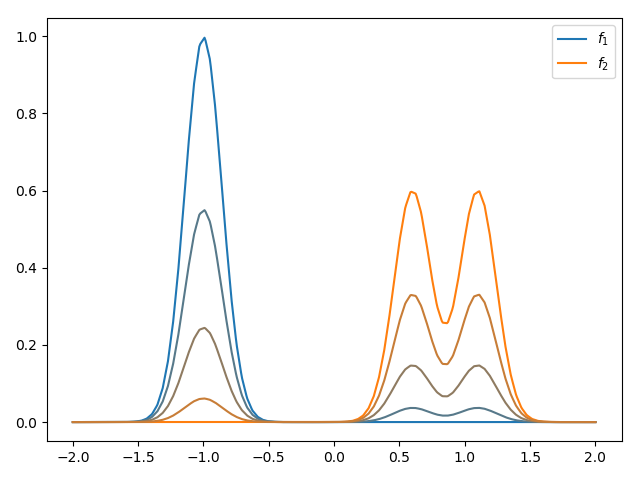
\includegraphics[width=7.5cm]{geodesic}} \quad
  \subfigure[SBFIG:GEODESIC2]{SRSF of the path}{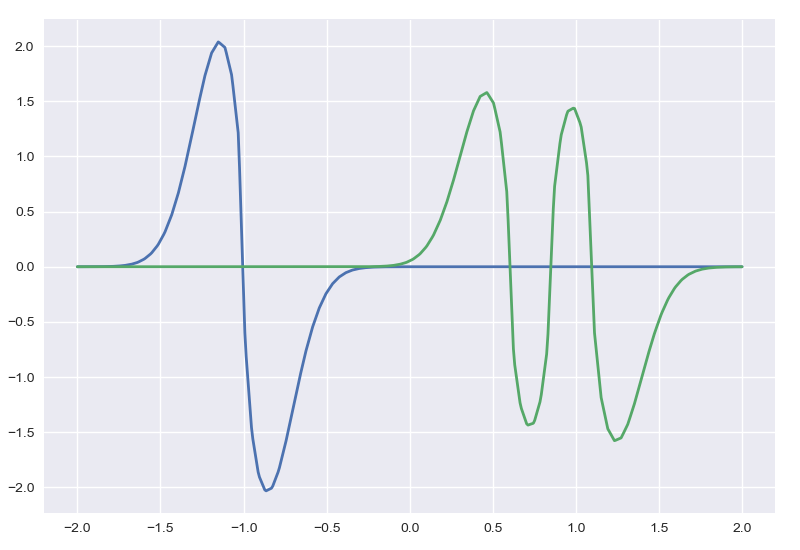
\includegraphics[width=7.5cm]{srsf-geodesic}}
\end{figure}

Given $f \in \mathcal{F}$, its \acs{SRSF} is defined as
$SRSF\{f\} = \operatorname{sgn}{(\dot f)} \sqrt{|\dot f|}$. To simplify notation, in the
subsequent sections, we will denote the  \acs{SRSF} of a function
$f_i \in \mathcal{F}$ as $q_i$.

Under this transformation, the Fisher-Rao metric becomes the usual metric
in $\mathbb{L}^2$, so that the distance between two functions will be
calculated using the distance $\mathbb{L}^2$ of their corresponding
SRSF's, i.e.,  $d_{FR}(f_1, f_2) = \| q_1 - q_2 \|_{\mathbb{L}^2}$. A proof of
this result is included in appendix \ref{SEC:ACTION}.

Taking advantage of this characterization we will take our functions to the
SRSFs space to perform the analysis efficiently, and then transform the result
to the original space. This can be done because the  \acs{SRSF} defines a map up to constant between
$\mathcal{F}$ and the space of SRSFs with the $\mathbb{L}^2$ metric.
A consequence is that the computation of geodesics shown in
\ref{FIG:GEODESIC} becomes in a straight line
between SRSFs,
$
\alpha(\tau) = (1 - \tau)q_1 + \tau q_2 \quad 0 \le \tau \le 1.
$

Given $\gamma \in \Gamma$, the SRSF of $f \circ \gamma$ is

\begin{equation}[]{SRSF of composition}
SRSF\{f \circ \gamma\} = \operatorname{sgn}(\dot{f} \circ \gamma) \sqrt{|\dot f \circ \gamma|}
\sqrt{\dot \gamma} = (q \circ \gamma) \sqrt{\dot \gamma}.
\end{equation}

To simplify the
notation, the  \acs{SRSF} of this composition is denoted by $(q, \gamma)$.
Using this fact, we can proof that the action of $\Gamma$ on $\mathcal{F}$ is an
action by isometries, i.e, given $f  \in \mathcal{F}$ and $\gamma \in \Gamma$
the composition $f \circ \gamma$ preserves the metric.
A proof of this result is given in the appendix \ref{SEC:ACTION}.
Figure \ref{FIG:ACTIONS} shows a diagram with the action of the composition
in the different spaces.

\begin{figure}[Action of $\Gamma$]{FIG:ACTIONS}{Action of $\Gamma$}

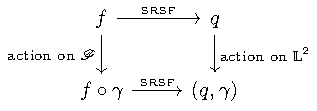
\includegraphics[width=8cm]{actions}

\end{figure}
